\section{Kontextabgrenzung}

Dieser Abschnitt beschreibt das Umfeld von PizzaPal. Für wen ist es da, und mit welchen Fremdsystemen interagiert es?

\subsection{Fachlicher Kontext}

\begin{figure}[H]
    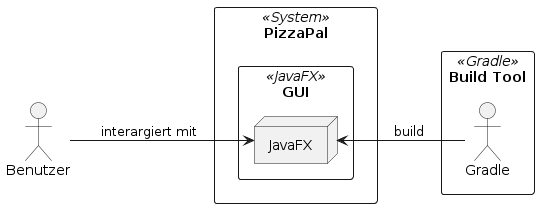
\includegraphics[width=\linewidth]{./images/kontextabgrenzung/kontextabgrenzung.png}
    \label{fig:fachKontext}
    \captionbelow{Fachlicher Kontext}
\end{figure}

\begin{longtable}{|m{0.3\textwidth}|m{0.7\textwidth}|}
    \hline
    \textbf{Nachbar} & \textbf{Beschreibung}\\
    \hline
    Benutzer & Gibt die zu sortierenden Zutaten über die GUI in das System ein. Das System überprüft die Eingabedaten auf Validität und zeigt die Ergebnisse auf der GUI entsprechend an.\\
    \hline
    Build Tool (Gradle) & Wird verwendet um die JavaFX-Anwendung zu bauen.\\
    \hline
\end{longtable}

\newpage
\subsection{Technischer Kontext}

\begin{figure}[H]
    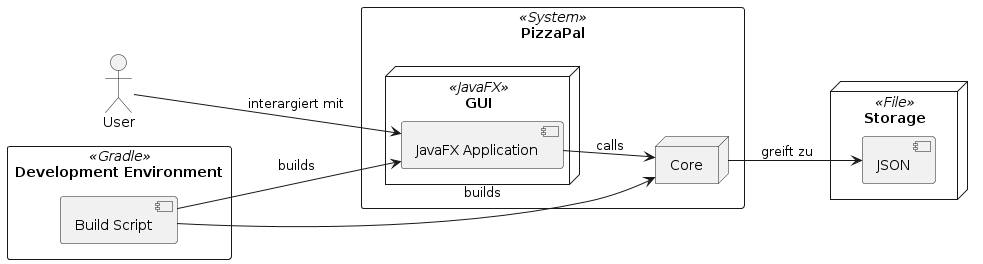
\includegraphics[width=\linewidth]{./images/kontextabgrenzung/kontextabgrenzungTech.png}
    \label{fig:techKontext}
    \captionbelow{Technischer Kontext}
\end{figure}

\begin{longtable}{|m{0.3\textwidth}|m{0.7\textwidth}|}
    \hline
    \textbf{Nachbar} & \textbf{Beschreibung}\\
    \hline
    Benutzer & Ein Akteur, der mit dem System interargiert.\\
    \hline
    Developer Environment(Gradle) & Entwicklungsrechner, der das Build-Script für das Gradle Plugin stellt. Wird verwendet um die Anwendung zu bauen.\\
    \hline
     JSON File &  Eine JSON-Datei, die als Speichermedium für Daten dient.\\
    \hline
    Core & Enthält die Geschäftslogik des Systems.\\
    \hline
\end{longtable}